\section{A Tour Through Tree RCU's Grace-Period Memory Ordering}
\label{sec:rcu:A Tour Through Tree RCU's Grace-Period Memory Ordering}

\begin{Note}
August 8, 2017

This article was contributed by Paul E. McKenney
\end{Note}

\subsection{Introduction}

This document gives a rough visual overview of how Tree RCU's
grace-period memory ordering guarantee is provided.

\subsection{What Is Tree RCU's Grace Period Memory Ordering Guarantee?}

RCU grace periods provide extremely strong memory-ordering guarantees
for non-idle non-offline code.
Any code that happens after the end of a given RCU grace period is guaranteed
to see the effects of all accesses prior to the beginning of that grace
period that are within RCU read-side critical sections.
Similarly, any code that happens before the beginning of a given RCU grace
period is guaranteed to not see the effects of all accesses following the end
of that grace period that are within RCU read-side critical sections.

Note well that RCU-sched read-side critical sections include any region
of code for which preemption is disabled.
Given that each individual machine instruction can be thought of as
an extremely small region of preemption-disabled code, one can think of
\co{synchronize_rcu()} as \co{smp_mb()} on steroids.

RCU updaters use this guarantee by splitting their updates into
two phases, one of which is executed before the grace period and
the other of which is executed after the grace period.
In the most common use case, phase one removes an element from
a linked RCU-protected data structure, and phase two frees that element.
For this to work, any readers that have witnessed state prior to the
phase-one update (in the common case, removal) must not witness state
following the phase-two update (in the common case, freeing).

The RCU implementation provides this guarantee using a network
of lock-based critical sections, memory barriers, and per-CPU
processing, as is described in the following sections.

\subsection{Tree RCU Grace Period Memory Ordering Building Blocks}

The workhorse for RCU's grace-period memory ordering is the
critical section for the \co{rcu_node} structure's
\co{->lock}.
These critical sections use helper functions for lock
acquisition, including \co{raw_spin_lock_rcu_node()},
\co{raw_spin_lock_irq_rcu_node()}, and \co{raw_spin_lock_irqsave_rcu_node()}.
Their lock-release counterparts are \co{raw_spin_unlock_rcu_node()},
\co{raw_spin_unlock_irq_rcu_node()}, and
\co{raw_spin_unlock_irqrestore_rcu_node()}, respectively.
For completeness, a \co{raw_spin_trylock_rcu_node()} is also provided.
The key point is that the lock-acquisition functions, including
\co{raw_spin_trylock_rcu_node()}, all invoke \co{smp_mb__after_unlock_lock()}
immediately after successful acquisition of the lock.

Therefore, for any given \co{rcu_node} structure, any access
happening before one of the above lock-release functions will be seen
by all CPUs as happening before any access happening after a later
one of the above lock-acquisition functions.
Furthermore, any access happening before one of the
above lock-release function on any given CPU will be seen by all
CPUs as happening before any access happening after a later one
of the above lock-acquisition functions executing on that same CPU,
even if the lock-release and lock-acquisition functions are operating
on different \co{rcu_node} structures.
Tree RCU uses these two ordering guarantees to form an ordering
network among all CPUs that were in any way involved in the grace
period, including any CPUs that came online or went offline during
the grace period in question.

The following litmus test exhibits the ordering effects of these
lock-acquisition and lock-release functions:

\begin{VerbatimN}
	int x, y, z;

	void task0(void)
	{
		raw_spin_lock_rcu_node(rnp);
		WRITE_ONCE(x, 1);
		r1 = READ_ONCE(y);
		raw_spin_unlock_rcu_node(rnp);
	}

	void task1(void)
	{
		raw_spin_lock_rcu_node(rnp);
		WRITE_ONCE(y, 1);
		r2 = READ_ONCE(z);
		raw_spin_unlock_rcu_node(rnp);
	}

	void task2(void)
	{
		WRITE_ONCE(z, 1);
		smp_mb();
		r3 = READ_ONCE(x);
	}

	WARN_ON(r1 == 0 && r2 == 0 && r3 == 0);
\end{VerbatimN}

The \co{WARN_ON()} is evaluated at ``the end of time'',
after all changes have propagated throughout the system.
Without the \co{smp_mb__after_unlock_lock()} provided by the
acquisition functions, this \co{WARN_ON()} could trigger, for example
on PowerPC\@.
The \co{smp_mb__after_unlock_lock()} invocations prevent this
\co{WARN_ON()} from triggering.

\QuickQuiz{
  But the chain of \co{rcu_node}-structure lock acquisitions guarantees
  that new readers will see all of the updater's pre-grace-period
  accesses and also guarantees that the updater's post-grace-period
  accesses will see all of the old reader's accesses.
  So why do we
  need all of those calls to \co{smp_mb__after_unlock_lock()}?
}\QuickQuizAnswer{
  Because we must provide ordering for RCU's polling grace-period
  primitives, for example, \co{get_state_synchronize_rcu()} and
  \co{poll_state_synchronize_rcu()}.
  Consider this code:

\begin{VerbatimU}
   CPU 0                                     CPU 1
   -----                                     -----
   WRITE_ONCE(X, 1)                          WRITE_ONCE(Y, 1)
   g = get_state_synchronize_rcu()           smp_mb()
   while (!poll_state_synchronize_rcu(g))    r1 = READ_ONCE(X)
          continue;
   r0 = READ_ONCE(Y)
\end{VerbatimU}

  RCU guarantees that the outcome \qco{r0 == 0 && r1 == 0} will not
  happen, even if CPU~1 is in an RCU extended quiescent state
  (idle or offline) and thus won't interact directly with the RCU
  core processing at all.
}\QuickQuizEnd

This approach must be extended to include idle CPUs, which need
RCU's grace-period memory ordering guarantee to extend to any
RCU read-side critical sections preceding and following the current
idle sojourn.
This case is handled by calls to the strongly ordered
\co{atomic_add_return()} read-modify-write atomic operation that
is invoked within \co{ct_kernel_exit_state()} at idle-entry
time and within \co{ct_kernel_enter_state()} at idle-exit time.
The grace-period kthread invokes first \co{ct_rcu_watching_cpu_acquire()}
(preceded by a full memory barrier) and \co{rcu_watching_snap_stopped_since()}
(both of which rely on acquire semantics) to detect idle CPUs.

\QuickQuiz{
  But what about CPUs that remain offline for the entire grace period?
}\QuickQuizAnswer{
  Such CPUs will be offline at the beginning of the grace period, so
  the grace period won't expect quiescent states from them.
  Races
  between grace-period start and CPU-hotplug operations are mediated
  by the CPU's leaf \co{rcu_node} structure's \co{->lock} as described
  above.
}\QuickQuizEnd

The approach must be extended to handle one final case, that of waking a
task blocked in \co{synchronize_rcu()}.
This task might be affined to
a CPU that is not yet aware that the grace period has ended, and thus
might not yet be subject to the grace period's memory ordering.
Therefore, there is an \co{smp_mb()} after the return from
\co{wait_for_completion()} in the \co{synchronize_rcu()} code path.

\QuickQuiz{
  What?
  Where???
  I don't see any \co{smp_mb()} after the return from
  \co{wait_for_completion()}!!!
}\QuickQuizAnswer{
  That would be because I spotted the need for that \co{smp_mb()} during
  the creation of this documentation, and it is therefore unlikely to
  hit mainline before v4.14.
  Kudos to Lance Roy, Will Deacon, Peter
  Zijlstra, and Jonathan Cameron for asking questions that sensitized
  me to the rather elaborate sequence of events that demonstrate the
  need for this memory barrier.
}\QuickQuizEnd

Tree RCU's grace-period memory-ordering guarantees rely most heavily on
the \co{rcu_node} structure's \co{->lock} field, so much so that it is
necessary to abbreviate this pattern in the diagrams in the next
section.
For example, consider the \co{rcu_prepare_for_idle()} function
shown below, which is one of several functions that enforce ordering of
newly arrived RCU callbacks against future grace periods:

\begin{fcvlabel}[ln:rcu:prepare-for-idle]
\begin{VerbatimN}[commandchars=\%\@\$]
	static void rcu_prepare_for_idle(void)
	{
		bool needwake;
		struct rcu_data *rdp = this_cpu_ptr(&rcu_data);
		struct rcu_node *rnp;
		int tne;

		lockdep_assert_irqs_disabled();
		if (rcu_rdp_is_offloaded(rdp))
			return;

		/* Handle nohz enablement switches conservatively. */
		tne = READ_ONCE(tick_nohz_active);
		if (tne != rdp->tick_nohz_enabled_snap) {
			if (!rcu_segcblist_empty(&rdp->cblist))
				invoke_rcu_core(); /* force nohz to see update. */
			rdp->tick_nohz_enabled_snap = tne;
			return;
		}
		if (!tne)
			return;

		/*
		 * If we have not yet accelerated this jiffy, accelerate all
		 * callbacks on this CPU.
		 */
		if (rdp->last_accelerate == jiffies)
			return;
		rdp->last_accelerate = jiffies;
		if (rcu_segcblist_pend_cbs(&rdp->cblist)) { %lnlbl@matters:b$
			rnp = rdp->mynode;
			raw_spin_lock_rcu_node(rnp); /* irqs already disabled. */ %lnlbl@matters:e$
			needwake = rcu_accelerate_cbs(rnp, rdp);
			raw_spin_unlock_rcu_node(rnp); /* irqs remain disabled. */
			if (needwake)
				rcu_gp_kthread_wake();
		}
	}
\end{VerbatimN}
\end{fcvlabel}

\begin{fcvref}[ln:rcu:prepare-for-idle:matters]
But the only part of \co{rcu_prepare_for_idle()} that really matters for
this discussion are \clnrefrange{b}{e}. % lines 32–34
\end{fcvref}
We will therefore abbreviate this
function as follows:

\begin{center}
\resizebox{.3\columnwidth}{!}{
\includegraphics{rcu/design/rcu_node-lock}}
\end{center}

The box represents the \co{rcu_node} structure's \co{->lock} critical
section, with the double line on top representing the additional
\co{smp_mb__after_unlock_lock()}.

\subsection{Tree RCU Grace Period Memory Ordering Components}

Tree RCU's grace-period memory-ordering guarantee is provided by a
number of RCU components:

\begin{enumerate}
\item Callback Registry
\item Grace-Period Initialization
\item Self-Reported Quiescent States
\item Dynamic Tick Interface
\item CPU-Hotplug Interface
\item Forcing Quiescent States
\item Grace-Period Cleanup
\item Callback Invocation
\end{enumerate}

Each of the following section looks at the corresponding component in
detail.

\subsubsection{Callback Registry}
\label{sec:rcu:memorder:Callback Registry}

If RCU's grace-period guarantee is to mean anything at all, any access
that happens before a given invocation of \co{call_rcu()} must also
happen before the corresponding grace period.
The implementation of this
portion of RCU's grace period guarantee is shown in the following
figure:

\begin{center}
\resizebox{.85\columnwidth}{!}{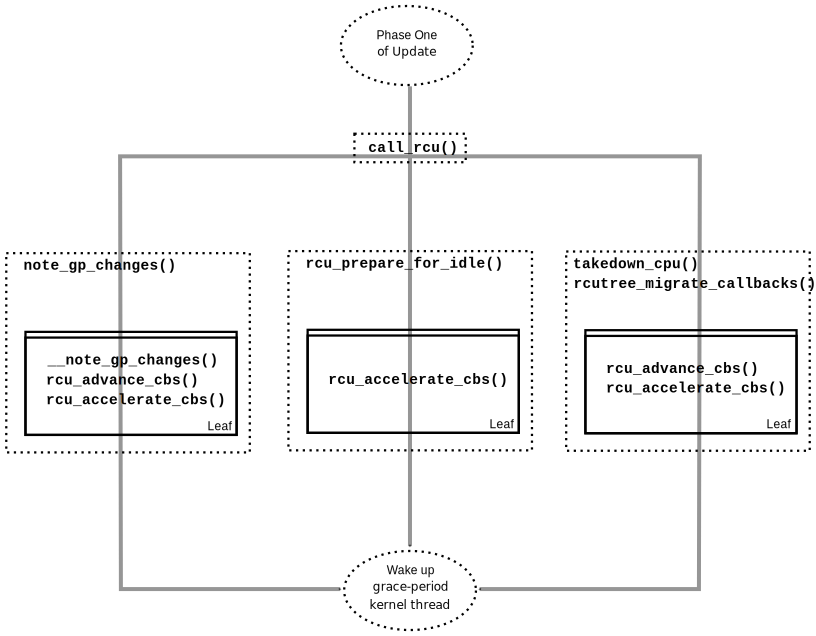
\includegraphics{rcu/design/TreeRCU-callback-registry}}
\end{center}

Because \co{call_rcu()} normally acts only on CPU-local state, it
provides no ordering guarantees, either for itself or for phase one of
the update (which again will usually be removal of an element from an
RCU-protected data structure).
It simply enqueues the \co{rcu_head}
structure on a per-CPU list, which cannot become associated with a grace
period until a later call to \co{rcu_accelerate_cbs()}, as shown in the
diagram above.

One set of code paths shown on the left invokes \co{rcu_accelerate_cbs()}
via \co{note_gp_changes()}, either directly from \co{call_rcu()} (if the
current CPU is inundated with queued \co{rcu_head} structures) or more
likely from an \co{RCU_SOFTIRQ} handler.
Another code path in the middle
is taken only in kernels built with \co{CONFIG_RCU_FAST_NO_HZ=y}, which
invokes \co{rcu_accelerate_cbs()} via \co{rcu_prepare_for_idle()}.
The
final code path on the right is taken only in kernels built with
\co{CONFIG_HOTPLUG_CPU=y}, which invokes \co{rcu_accelerate_cbs()} via
\co{rcu_advance_cbs()}, \co{rcu_migrate_callbacks},
\co{rcutree_migrate_callbacks()}, and \co{takedown_cpu()}, which in turn
is invoked on a surviving CPU after the outgoing CPU has been completely
offlined.

There are a few other code paths within grace-period processing that
opportunistically invoke \co{rcu_accelerate_cbs()}.
However, either way,
all of the CPU's recently queued \co{rcu_head} structures are associated
with a future grace-period number under the protection of the CPU's lead
\co{rcu_node} structure's \co{->lock}.
In all cases, there is full
ordering against any prior critical section for that same \co{rcu_node}
structure's \co{->lock}, and also full ordering against any of the
current task's or CPU's prior critical sections for any \co{rcu_node}
structure's \co{->lock}.

The next section will show how this ordering ensures that any accesses
prior to the \co{call_rcu()} (particularly including phase one of the
update) happen before the start of the corresponding grace period.

\QuickQuiz{
  But what about \co{synchronize_rcu()}?
}\QuickQuizAnswer{
  The \co{synchronize_rcu()} passes \co{call_rcu()} to \co{wait_rcu_gp()},
  which invokes it.
  So either way, it eventually comes down to
  \co{call_rcu()}.
}\QuickQuizEnd

\subsubsection{Grace-Period Initialization}
\label{sec:rcu:memorder:Grace-Period Initialization}

Grace-period initialization is carried out by the grace-period kernel
thread, which makes several passes over the \co{rcu_node} tree within the
\co{rcu_gp_init()} function.
This means that showing the full flow of
ordering through the grace-period computation will require duplicating
this tree.
If you find this confusing, please note that the state of the
\co{rcu_node} changes over time, just like Heraclitus's river.
However,
to keep the \co{rcu_node} river tractable, the grace-period kernel
thread's traversals are presented in multiple parts, starting in this
section with the various phases of grace-period initialization.

The first ordering-related grace-period initialization action is to
advance the \co{rcu_state} structure's \co{->gp_seq} grace-period-number
counter, as shown below:

\begin{center}
\resizebox{\columnwidth}{!}{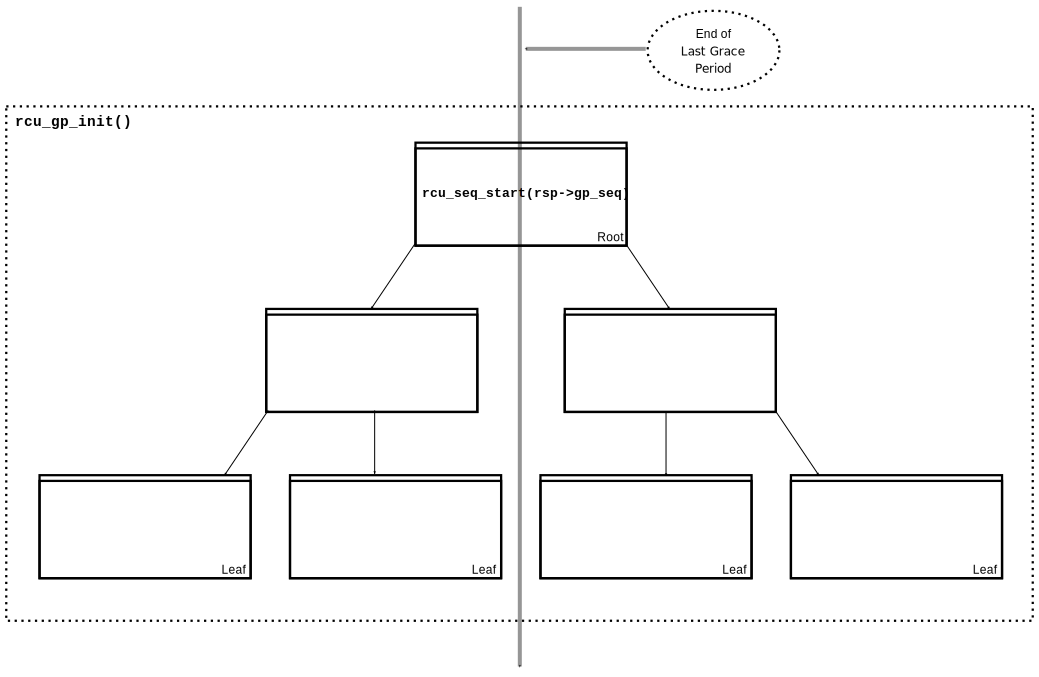
\includegraphics{rcu/design/TreeRCU-gp-init-1}}
\end{center}

The actual increment is carried out using \co{smp_store_release()}, which
helps reject false-positive RCU CPU stall detection. Note that only the
root \co{rcu_node} structure is touched.

The first pass through the \co{rcu_node} tree updates bitmasks based on
CPUs having come online or gone offline since the start of the previous
grace period.
In the common case where the number of online CPUs for
this \co{rcu_node} structure has not transitioned to or from zero, this
pass will scan only the leaf \co{rcu_node} structures.
However, if the
number of online CPUs for a given leaf \co{rcu_node} structure has
transitioned from zero, \co{rcu_init_new_rnp()} will be invoked for the
first incoming CPU\@.
Similarly, if the number of online CPUs for a given
leaf \co{rcu_node} structure has transitioned to zero,
\co{rcu_cleanup_dead_rnp()} will be invoked for the last outgoing CPU\@.
The diagram below shows the path of ordering if the leftmost
\co{rcu_node} structure onlines its first CPU and if the next
\co{rcu_node} structure has no online CPUs (or, alternatively if the
leftmost \co{rcu_node} structure offlines its last CPU and if the next
\co{rcu_node} structure has no online CPUs).

\begin{center}
\resizebox{\columnwidth}{!}{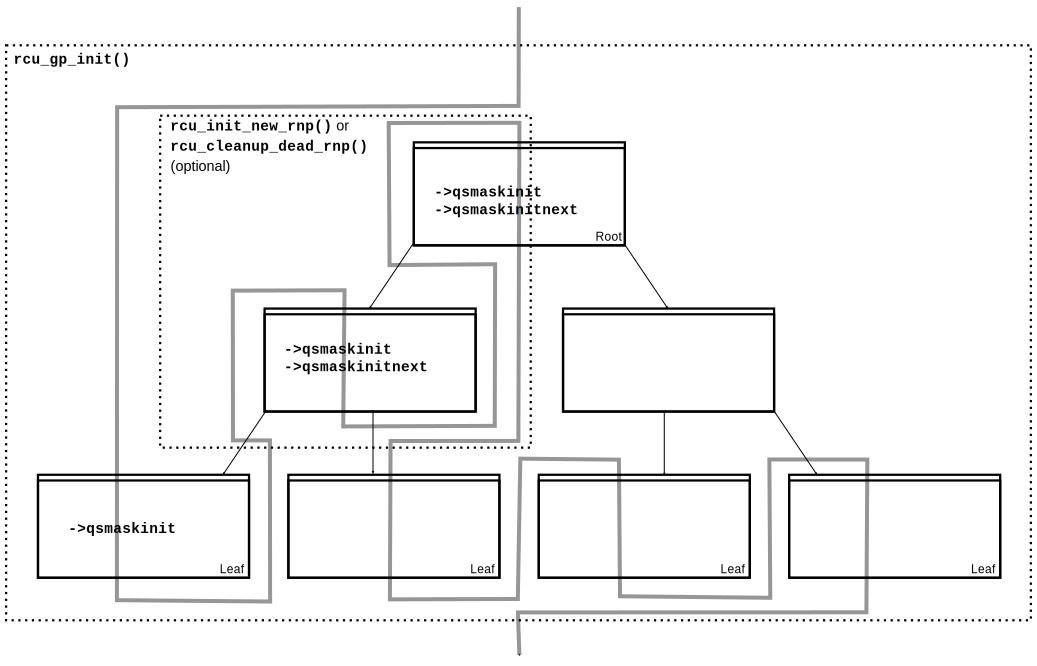
\includegraphics{rcu/design/TreeRCU-gp-init-2}}
\end{center}

The final \co{rcu_gp_init()} pass through the \co{rcu_node} tree traverses
breadth-first, setting each \co{rcu_node} structure's \co{->gp_seq} field
to the newly advanced value from the \co{rcu_state} structure, as shown
in the following diagram.

\begin{center}
\resizebox{\columnwidth}{!}{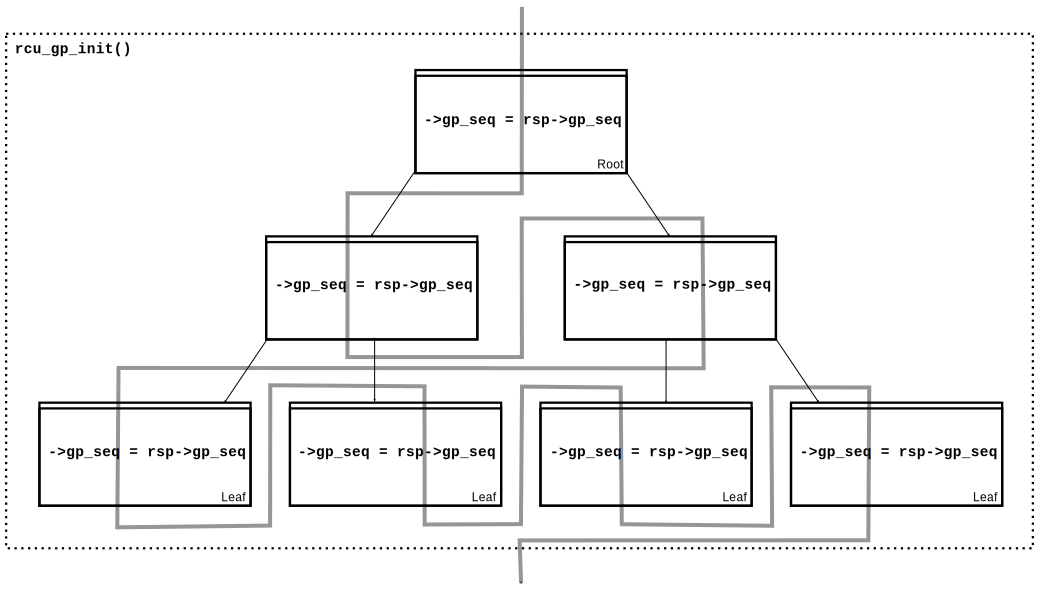
\includegraphics{rcu/design/TreeRCU-gp-init-3}}
\end{center}

This change will also cause each CPU's next call to
\co{__note_gp_changes()} to notice that a new grace period has started,
as described in the next section.
But because the grace-period kthread
started the grace period at the root (with the advancing of the
\co{rcu_state} structure's \co{->gp_seq} field) before setting each leaf
\co{rcu_node} structure's \co{->gp_seq} field, each CPU's observation of
the start of the grace period will happen after the actual start of the
grace period.

\QuickQuiz{
  But what about the CPU that started the grace period? Why wouldn't it
  see the start of the grace period right when it started that grace
  period?
}\QuickQuizAnswer{
  In some deep philosophical and overly anthromorphized sense, yes, the
  CPU starting the grace period is immediately aware of having done so.
  However, if we instead assume that RCU is not self-aware, then even
  the CPU starting the grace period does not really become aware of the
  start of this grace period until its first call to
  \co{__note_gp_changes()}.
  On the other hand, this CPU potentially gets
  early notification because it invokes \co{__note_gp_changes()} during
  its last \co{rcu_gp_init()} pass through its leaf \co{rcu_node}
  structure.
}\QuickQuizEnd

\subsubsection{Self-Reported Quiescent States}
\label{sec:rcu:memorder:Self-Reported Quiescent States}

When all entities that might block the grace period have reported
quiescent states (or as described in a later section, had quiescent
states reported on their behalf), the grace period can end. Online
non-idle CPUs report their own quiescent states, as shown in the
following diagram:

\begin{center}
\resizebox{\columnwidth}{!}{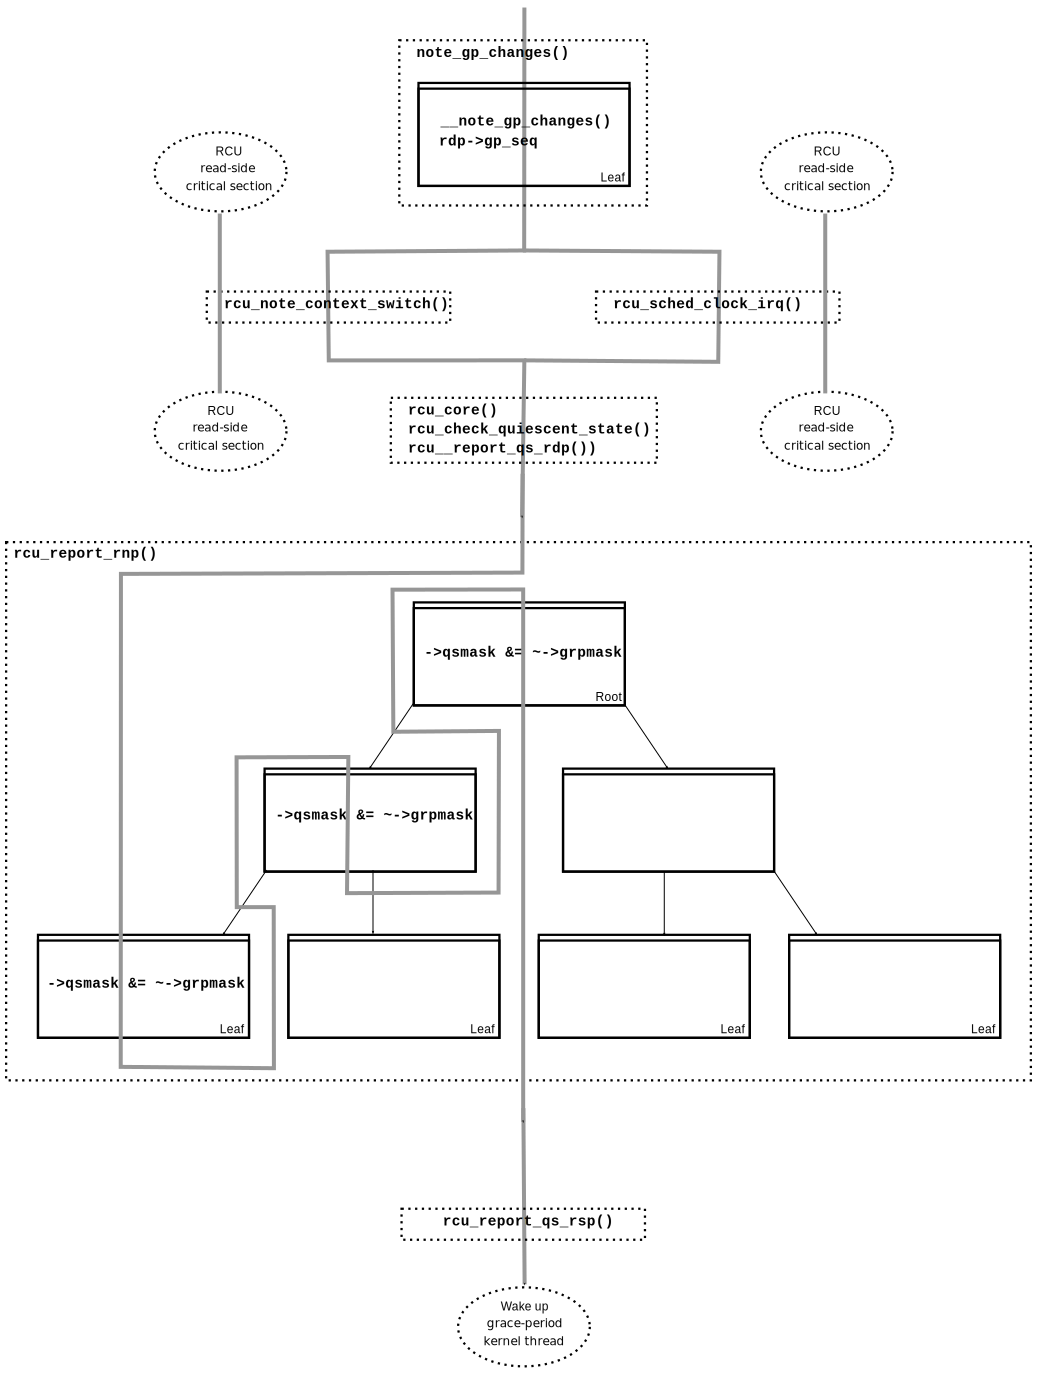
\includegraphics{rcu/design/TreeRCU-qs}}
\end{center}

This is for the last CPU to report a quiescent state, which signals the
end of the grace period. Earlier quiescent states would push up the
\co{rcu_node} tree only until they encountered an \co{rcu_node} structure
that is waiting for additional quiescent states.
However, ordering is
nevertheless preserved because some later quiescent state will acquire
that \co{rcu_node} structure's \co{->lock}.

Any number of events can lead up to a CPU invoking \co{note_gp_changes}
(or alternatively, directly invoking \co{__note_gp_changes()}), at which
point that CPU will notice the start of a new grace period while holding
its leaf \co{rcu_node} lock.
Therefore, all execution shown in this
diagram happens after the start of the grace period.
In addition, this
CPU will consider any RCU read-side critical section that started before
the invocation of \co{__note_gp_changes()} to have started before the
grace period, and thus a critical section that the grace period must
wait on.

\QuickQuiz{
  But a RCU read-side critical section might have started after the
  beginning of the grace period (the advancing of \co{->gp_seq} from
  earlier), so why should the grace period wait on such a critical
  section?
}\QuickQuizAnswer{
  It is indeed not necessary for the grace period to wait on such a
  critical section.
  However, it is permissible to wait on it. And it is
  furthermore important to wait on it, as this lazy approach is far
  more scalable than a ``big bang'' all-at-once grace-period start could
  possibly be.
}\QuickQuizEnd

If the CPU does a context switch, a quiescent state will be noted by
\co{rcu_note_context_switch()} on the left.
On the other hand, if the CPU
takes a scheduler-clock interrupt while executing in usermode, a
quiescent state will be noted by \co{rcu_sched_clock_irq()} on the right.
Either way, the passage through a quiescent state will be noted in a
per-CPU variable.

The next time an \co{RCU_SOFTIRQ} handler executes on this CPU (for
example, after the next scheduler-clock interrupt), \co{rcu_core()} will
invoke \co{rcu_check_quiescent_state()}, which will notice the recorded
quiescent state, and invoke \co{rcu_report_qs_rdp()}.
If
\co{rcu_report_qs_rdp()} verifies that the quiescent state really does
apply to the current grace period, it invokes \co{rcu_report_rnp()} which
traverses up the \co{rcu_node} tree as shown at the bottom of the
diagram, clearing bits from each \co{rcu_node} structure's \co{->qsmask}
field, and propagating up the tree when the result is zero.

Note that traversal passes upwards out of a given \co{rcu_node} structure
only if the current CPU is reporting the last quiescent state for the
subtree headed by that \co{rcu_node} structure.
A key point is that if a
CPU's traversal stops at a given \co{rcu_node} structure, then there will
be a later traversal by another CPU (or perhaps the same one) that
proceeds upwards from that point, and the \co{rcu_node} \co{->lock}
guarantees that the first CPU's quiescent state happens before the
remainder of the second CPU's traversal.
Applying this line of thought
repeatedly shows that all CPUs' quiescent states happen before the last
CPU traverses through the root \co{rcu_node} structure, the ``last CPU''
being the one that clears the last bit in the root \co{rcu_node}
structure's \co{->qsmask} field.

\subsubsection{Dynamic Tick Interface}
\label{sec:rcu:memorder:Dynamic Tick Interface}

Due to energy-efficiency considerations, RCU is forbidden from
disturbing idle CPUs.
CPUs are therefore required to notify RCU when
entering or leaving idle state, which they do via fully ordered
value-returning atomic operations on a per-CPU variable.
The ordering
effects are as shown below:

\begin{center}
\resizebox{.7\columnwidth}{!}{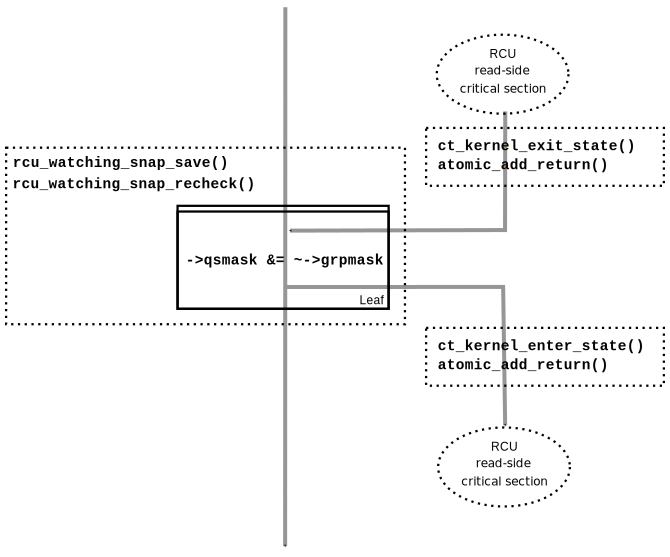
\includegraphics{rcu/design/TreeRCU-dyntick}}
\end{center}

The RCU grace-period kernel thread samples the per-CPU idleness variable
while holding the corresponding CPU's leaf \co{rcu_node} structure's
\co{->lock}.
This means that any RCU read-side critical sections that
precede the idle period (the oval near the top of the diagram above)
will happen before the end of the current grace period. Similarly, the
beginning of the current grace period will happen before any RCU
read-side critical sections that follow the idle period (the oval near
the bottom of the diagram above).

Plumbing this into the full grace-period execution is described below
in \cref{sec:rcu:memorder:Forcing Quiescent States}.


\subsubsection{CPU-Hotplug Interface}
\label{sec:rcu:memorder:CPU-Hotplug Interface}

RCU is also forbidden from disturbing offline CPUs, which might well be
powered off and removed from the system completely.
CPUs are therefore
required to notify RCU of their comings and goings as part of the
corresponding CPU hotplug operations.
The ordering effects are shown
below:

\begin{center}
\resizebox{.6\columnwidth}{!}{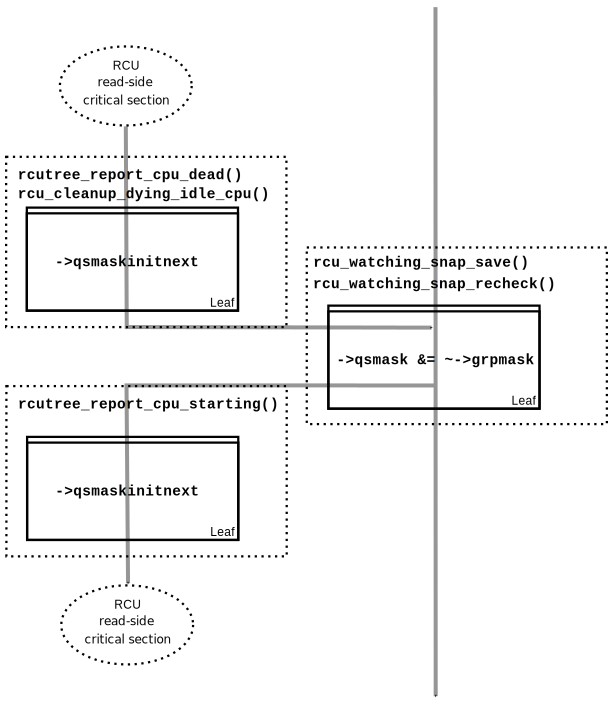
\includegraphics{rcu/design/TreeRCU-hotplug}}
\end{center}

Because CPU hotplug operations are much less frequent than idle
transitions, they are heavier weight, and thus acquire the CPU's leaf
\co{rcu_node} structure's \co{->lock} and update this structure's
\co{->qsmaskinitnext}.
The RCU grace-period kernel thread samples this
mask to detect CPUs having gone offline since the beginning of this
grace period.

Plumbing this into the full grace-period execution is described below
in \cref{sec:rcu:memorder:Forcing Quiescent States}.


\subsubsection{Forcing Quiescent States}
\label{sec:rcu:memorder:Forcing Quiescent States}

As noted above, idle and offline CPUs cannot report their own quiescent
states, and therefore the grace-period kernel thread must do the
reporting on their behalf.
This process is called ``forcing quiescent
states'', it is repeated every few jiffies, and its ordering effects are
shown below:

\begin{center}
\resizebox{\columnwidth}{!}{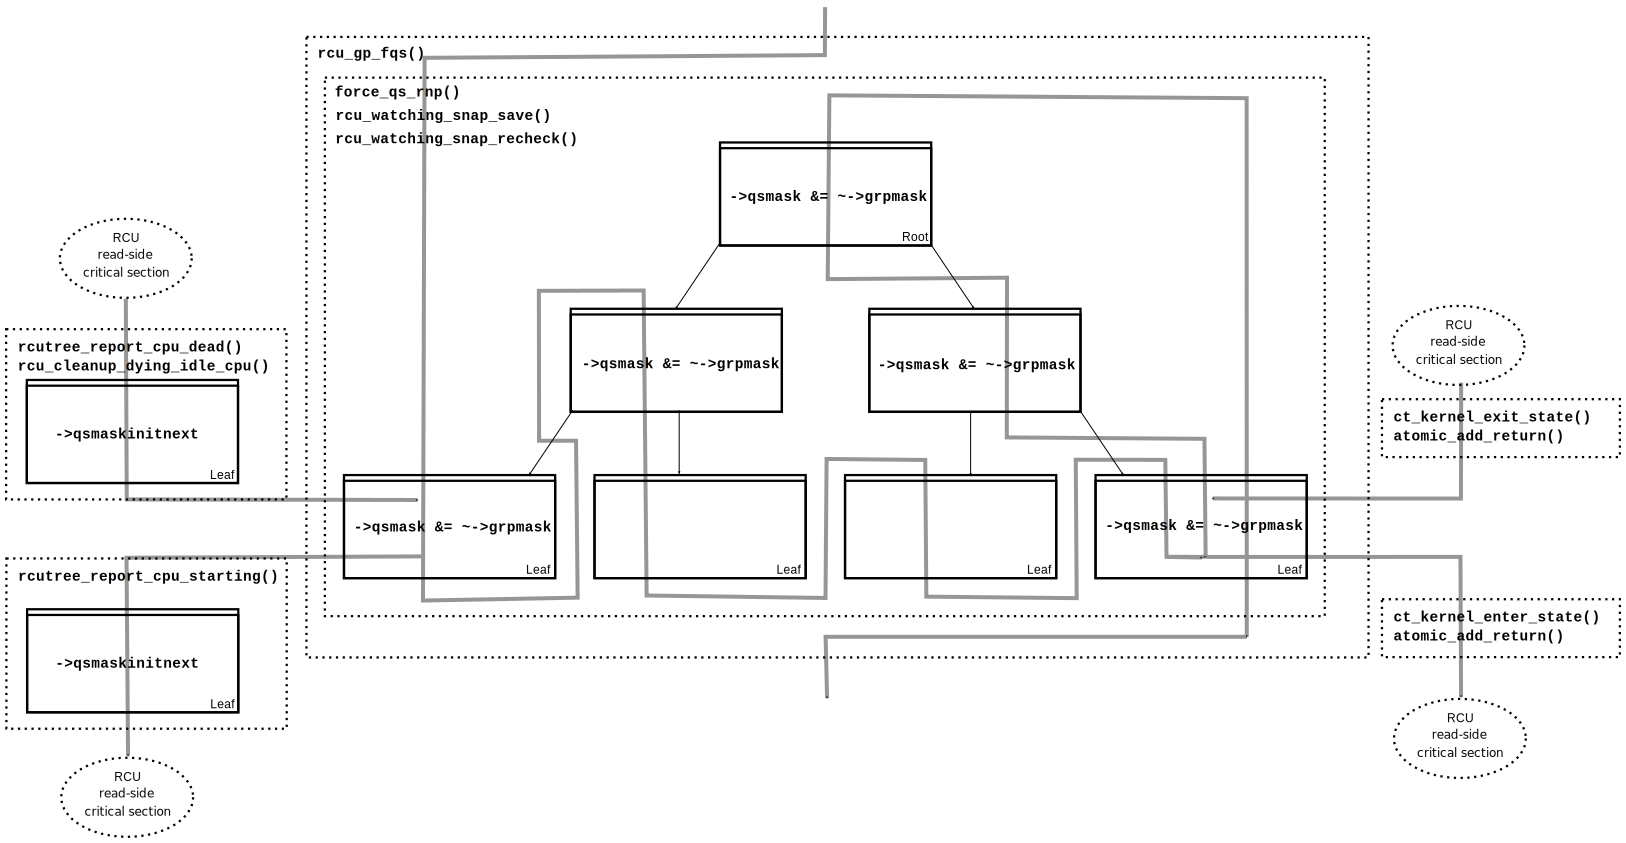
\includegraphics{rcu/design/TreeRCU-gp-fqs}}
\end{center}

Each pass of quiescent state forcing is guaranteed to traverse the leaf
\co{rcu_node} structures, and if there are no new quiescent states due to
recently idled and/or offlined CPUs, then only the leaves are traversed.
However, if there is a newly offlined CPU as illustrated on the left or
a newly idled CPU as illustrated on the right, the corresponding
quiescent state will be driven up towards the root.
As with
self-reported quiescent states, the upwards driving stops once it
reaches an \co{rcu_node} structure that has quiescent states outstanding
from other CPUs.

\QuickQuiz{
  The leftmost drive to root stopped before it reached the root
  \co{rcu_node} structure, which means that there are still CPUs
  subordinate to that structure on which the current grace period is
  waiting.
  Given that, how is it possible that the rightmost drive to
  root ended the grace period?
}\QuickQuizAnswer{
  Good analysis!
  It is in fact impossible in the absence of bugs in
  RCU\@. But this diagram is complex enough as it is, so simplicity
  overrode accuracy. You can think of it as poetic license, or you can
  think of it as misdirection that is resolved in the
  stitched-together diagram shown in
  \cref{sec:rcu:memorder:Putting It All Together}.
}\QuickQuizEnd


\subsubsection{Grace-Period Cleanup}
\label{sec:rcu:memorder:Grace-Period Cleanup}

Grace-period cleanup first scans the \co{rcu_node} tree breadth-first
advancing all the \co{->gp_seq} fields, then it advances the
\co{rcu_state} structure's \co{->gp_seq} field. The ordering effects are
shown below:

\begin{center}
\resizebox{.85\columnwidth}{!}{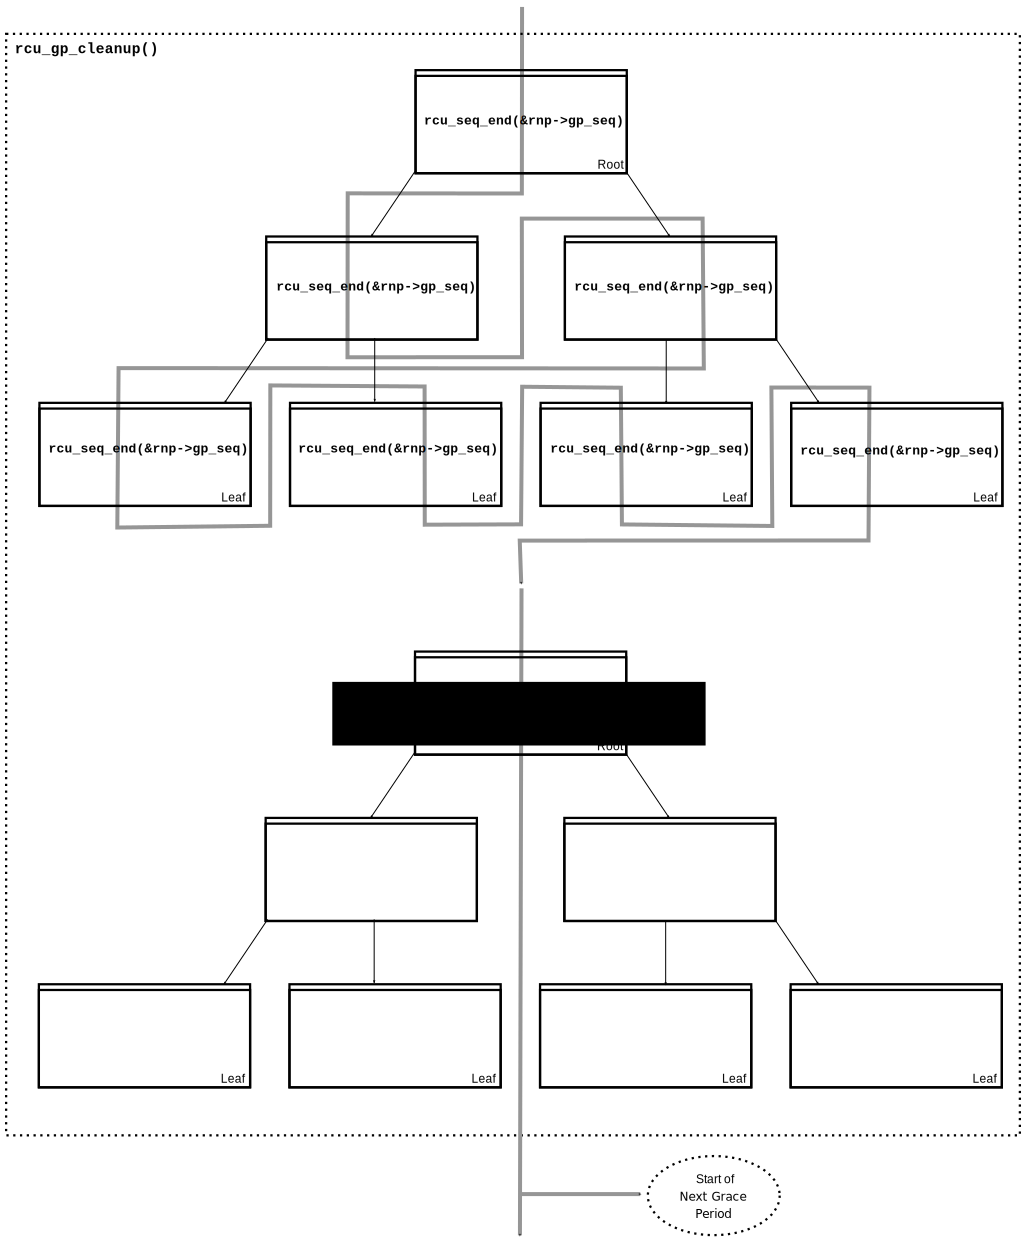
\includegraphics{rcu/design/TreeRCU-gp-cleanup}}
\end{center}

As indicated by the oval at the bottom of the diagram, once grace-period
cleanup is complete, the next grace period can begin.

\QuickQuiz{
  But when precisely does the grace period end?
}\QuickQuizAnswer{
  There is no useful single point at which the grace period can be said
  to end.
  The earliest reasonable candidate is as soon as the last CPU
  has reported its quiescent state, but it may be some milliseconds
  before RCU becomes aware of this.
  The latest reasonable candidate is
  once the \co{rcu_state} structure's \co{->gp_seq} field has been
  updated, but it is quite possible that some CPUs have already
  completed phase two of their updates by that time.
  In short, if you
  are going to work with RCU, you need to learn to embrace uncertainty.
}\QuickQuizEnd


\subsubsection{Callback Invocation}
\label{sec:rcu:memorder:Callback Invocation}

Once a given CPU's leaf \co{rcu_node} structure's \co{->gp_seq} field has
been updated, that CPU can begin invoking its RCU callbacks that were
waiting for this grace period to end.
These callbacks are identified by
\co{rcu_advance_cbs()}, which is usually invoked by
\co{__note_gp_changes()}.
As shown in the diagram below, this invocation
can be triggered by the scheduling-clock interrupt
(\co{rcu_sched_clock_irq()} on the left) or by idle entry
(\co{rcu_cleanup_after_idle()} on the right, but only for kernels build
with \co{CONFIG_RCU_FAST_NO_HZ=y}).
Either way, \co{RCU_SOFTIRQ} is
raised, which results in \co{rcu_do_batch()} invoking the callbacks,
which in turn allows those callbacks to carry out (either directly or
indirectly via wakeup) the needed phase-two processing for each update.

\begin{center}
\resizebox{.7\columnwidth}{!}{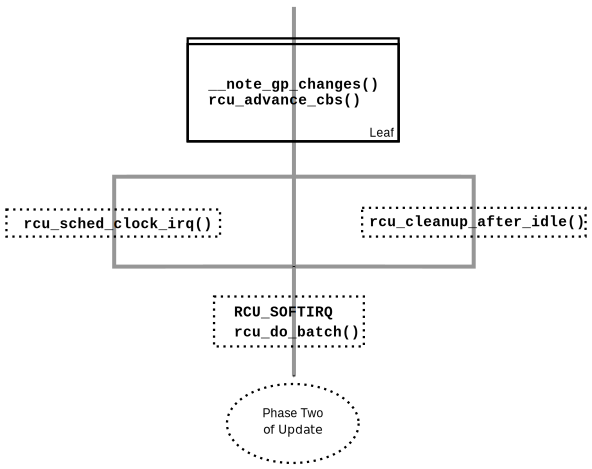
\includegraphics{rcu/design/TreeRCU-callback-invocation}}
\end{center}

Please note that callback invocation can also be prompted by any number
of corner-case code paths, for example, when a CPU notes that it has
excessive numbers of callbacks queued.
In all cases, the CPU acquires
its leaf \co{rcu_node} structure's \co{->lock} before invoking callbacks,
which preserves the required ordering against the newly completed grace
period.

However, if the callback function communicates to other CPUs, for
example, doing a wakeup, then it is that function's responsibility to
maintain ordering.
For example, if the callback function wakes up a task
that runs on some other CPU, proper ordering must in place in both the
callback function and the task being awakened.
To see why this is
important, consider the top half of the diagram shown above in
\cref{sec:rcu:memorder:Grace-Period Cleanup}.
The callback might be
running on a CPU corresponding to the leftmost leaf \co{rcu_node}
structure, and awaken a task that is to run on a CPU corresponding to
the rightmost leaf \co{rcu_node} structure, and the grace-period kernel
thread might not yet have reached the rightmost leaf.
In this case, the
grace period's memory ordering might not yet have reached that CPU, so
again the callback function and the awakened task must supply proper
ordering.

\subsubsection{Putting It All Together}
\label{sec:rcu:memorder:Putting It All Together}

A stitched-together diagram is here:

\begin{center}
\resizebox{.365\columnwidth}{!}{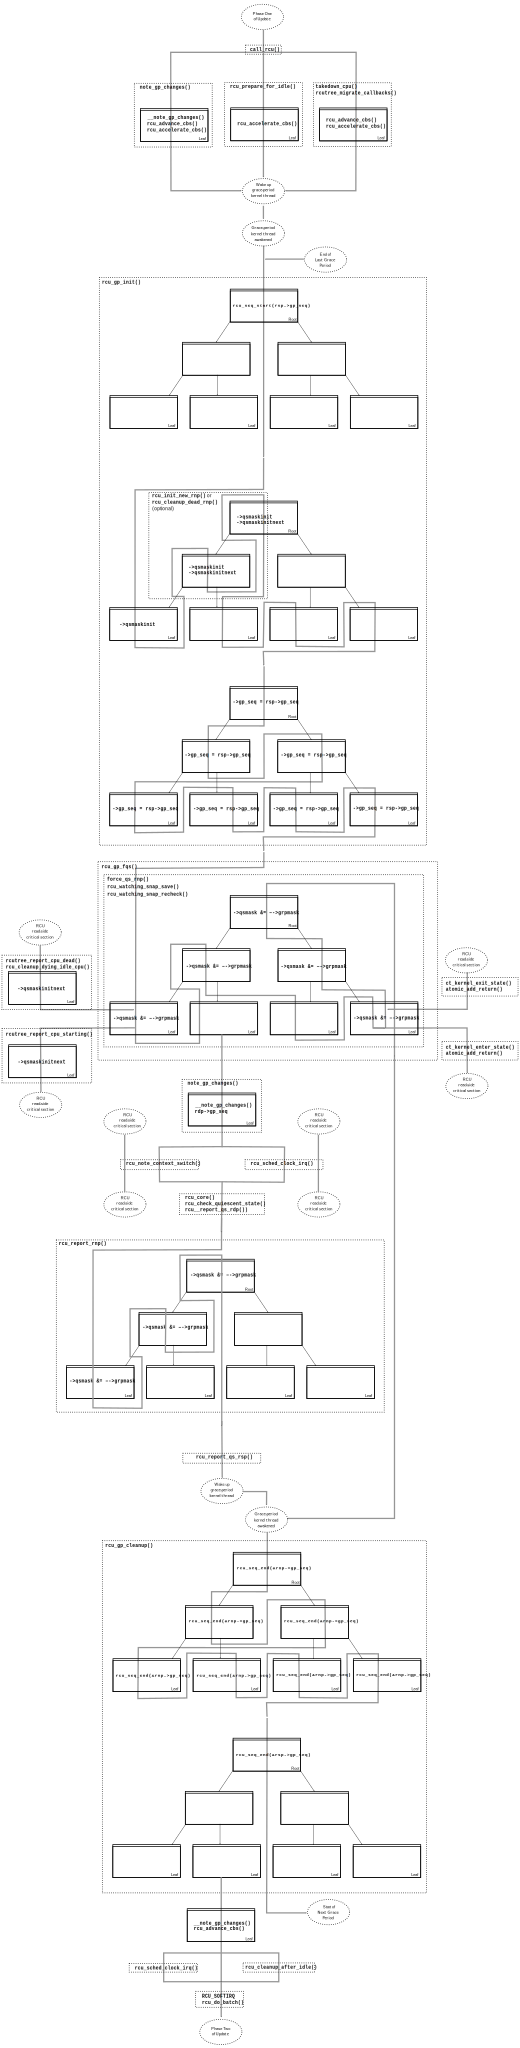
\includegraphics{rcu/design/TreeRCU-gp}}
\end{center}

\subsection{Legal Statement}

This work represents the view of the author and does not necessarily
represent the view of IBM\@.

Linux is a registered trademark of Linus Torvalds.

Other company, product, and service names may be trademarks or service
marks of others.
